\section{Applications}
\label{sec:apps}
In this section we discuss three applications we wrote that use the infrastructure we set up inside a building on campus.
The building is a 7-story, 141,000 square-foot building.  We tagged 351 items spread over 139 rooms throughout all floors.
There are WiFi access point spread throughout the entire building, providing ubiquitous access to a network throughout.
Cellular coverage is also available throughout most of the building as a secondary option for connecting to a network.

The first application we built is an energy auditing application.  The goal was to get a sense for how energy
was being used by the plug-loads distributed throughout the building.  We collected both power rating information as well
as live metering information.  The second application, the energy-view item scanner, builds off the first, allowing users
to swipe the QR code of an item and view the power-trace and power-rating recorded for that item.  It is also
used to view aggregates across space; you can scan a floor and see the aggregate data for that floor over time.  
The third is a personal energy accountant.  This application allows users to virtually tag items that belong to them 
and view their personal energy consumption, aggregated across all the devices they own.

\subsection{Energy Auditing}
\label{sec:eaudit}
The energy auditing application was written to capture all of the plug-load devices in a building.  Included it their
capture is information about the plated power-draw of the device, if available, its make, model, and category.
The capture consists of walking around the building with a set of QR codes, registering each of the rooms and items
within them.  For each room you enter the name of the room.  The floor is indicated explicitly through a swipe of the buidling
floor tag.  Once inside the room each electrical device is tagged and registered.  To register the item the QR code needs
to be added, followed by a small form that is filled out by the auditor.  The form includes information for the name
of the device and the power rating or current draw.  

Figure~\ref{fig:msfsv2} shows two screenshot of the auditing interface.  The first page is a list of options and the second is
the registration page.  Once the page is filled out, the user scans the QR code once again and the item is added to the inventory.
In addition, the QR code tag identifier is added to the `qrc' directory and symbolically linked to the newly added item
in the inventory directory.  Finally, a symbolic link is create in the directory for the room that also points to the item
just added to the inventory.

\begin{figure}[htb!]
\begin{center}
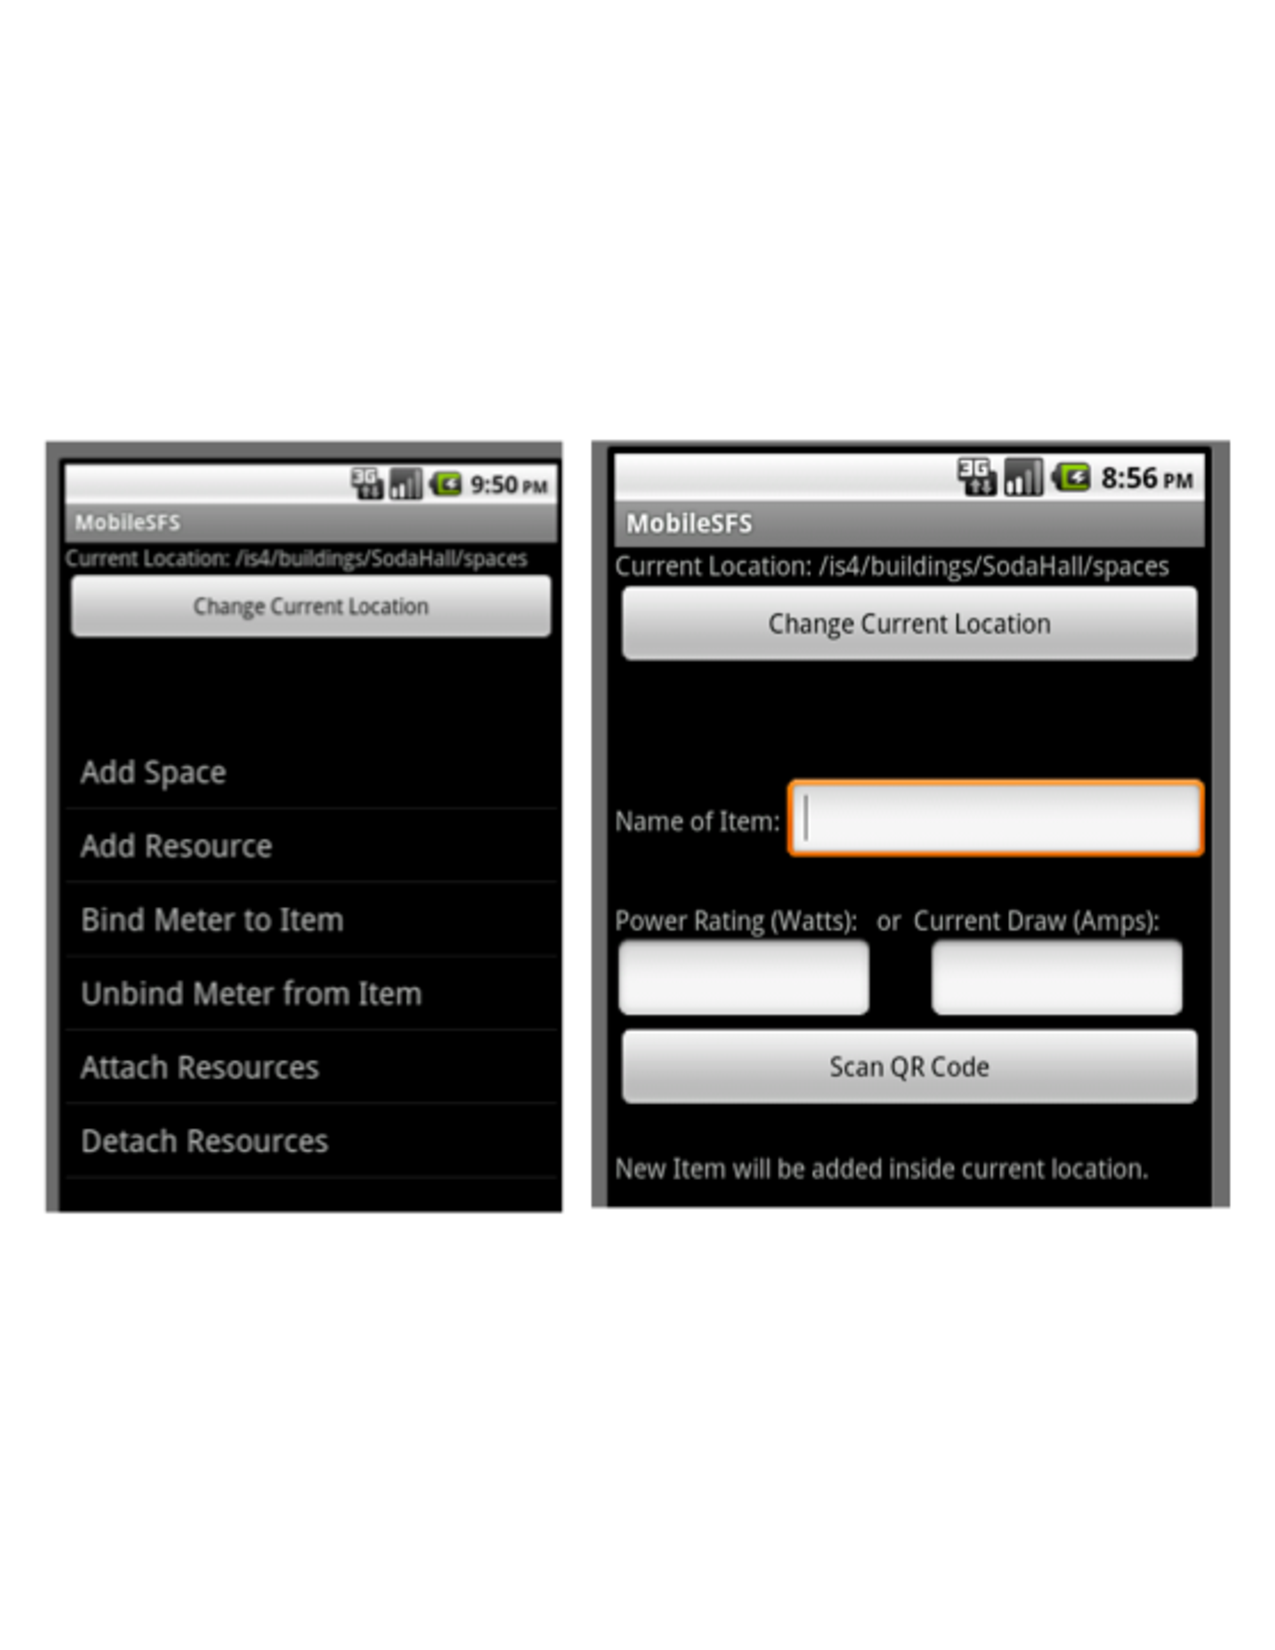
\includegraphics[scale=0.39]{figs/msfsv2screens}
\caption{}
\label{fig:msfsv2}
\end{center}
\end{figure}

Auto-classification was done using the same of the item as well.  In addition to the spaces, qrc, and inventory directories
there is also a taxonomony directory.  Items with a given prefix were classified as being items in a particular
directory of the taxonomy.  A symbolic link was also created from the corresponding node in the taxonomy, that most closely
matches the item, to the item node.

\subsubsection{Results}
This application was focused on capturing the physical, energy-consuming objects, describing them in various way
and coupling that information with live streaming power data.  Figure~\ref{fig:devicecount} shows the breakdown of the
types of devices that were recorded by the energy auditing application.  Since this data was collected from a office
building, most of the device were actually LCD screens.

\begin{figure}[htb!]
\begin{center}
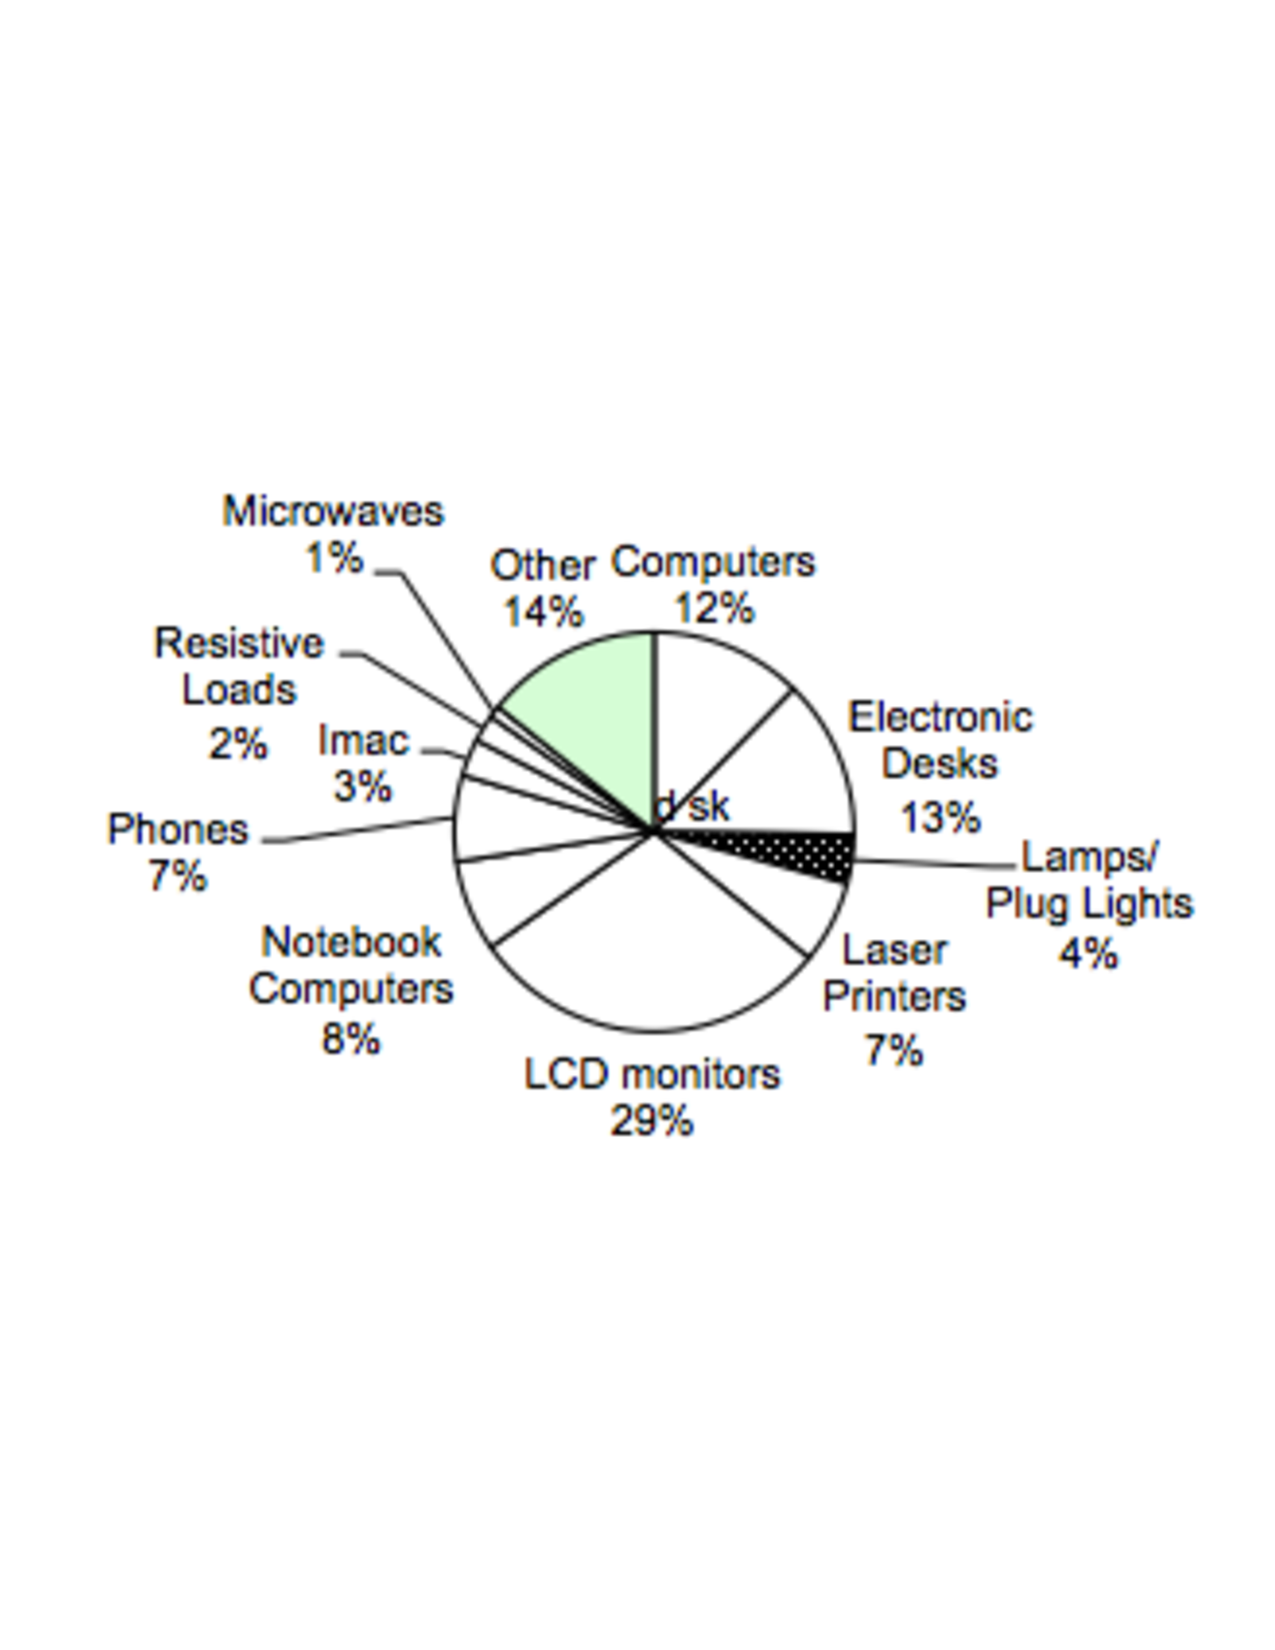
\includegraphics[scale=0.42]{figs/devicecount}
\caption{The percentage breakdown of the devices that were captured.}
\label{fig:devicecount}
\end{center}
\end{figure}

Although most of the items are static, a good number of them are moved by their owners pretty often.  For example, 8\%
of the device were classified as notebooks.  When the owner leaves the room or building, they usually take their notebook
with them.  This kind of information should be recorded using the auditing application.  By simply swiping QR code for the notebook
and clicking the `leave' button, the item is kept in the inventory for the building, but the symbolic link from the 
room to the item is deleted.

\begin{figure}[htb!]
\begin{center}
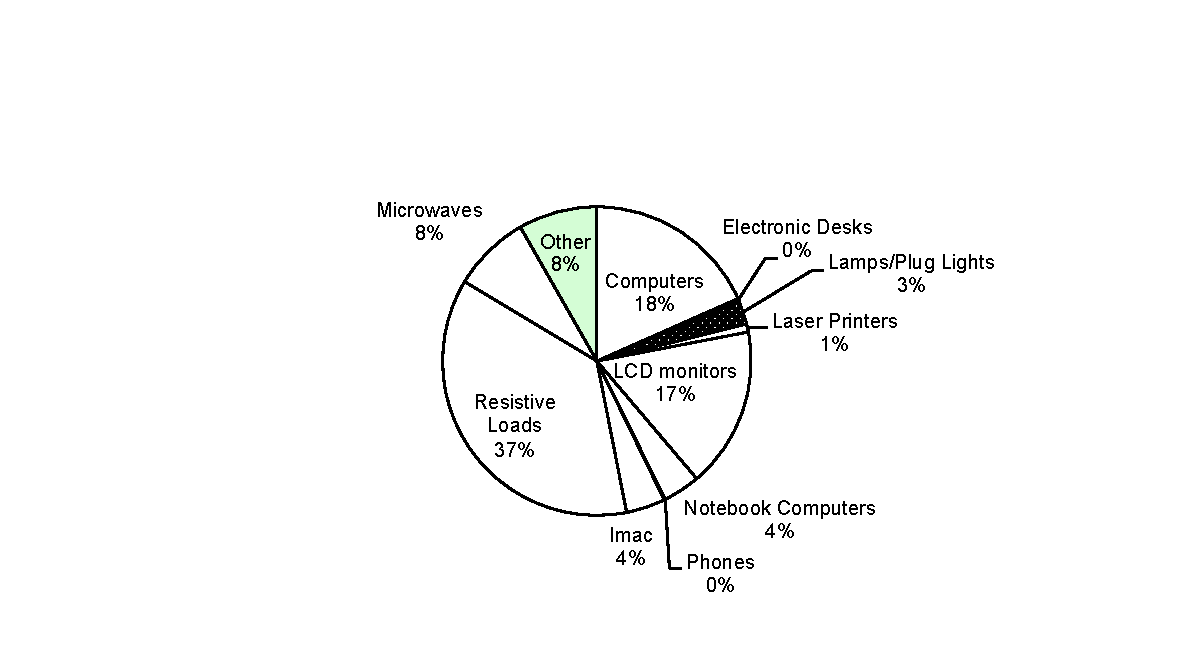
\includegraphics[scale=0.7]{figs/PIE_CHART_SANS_WATTS}
\caption{Device power draw in Watts.}
\label{fig:piechart}
\end{center}
\end{figure}

Figure~\ref{fig:piechart} shows the power-draw distribution.  Interestingly, although the category of devices that 
fall under `resistive loads' only make up 2\% of the items recorded, they account for 37\% of the total power-draw.
However, note that this is calculated with respect to the power-draw figure placed on the device itself.  It is not
based on measured power-draw.  This calculation was made using the properties that were inserted in StreamFS.
Each of the item nodes were recorded as having a certain power-draw and that was used to calculate the total the 
percentage of total according to each category.

\begin{figure}[htb!]
\begin{center}
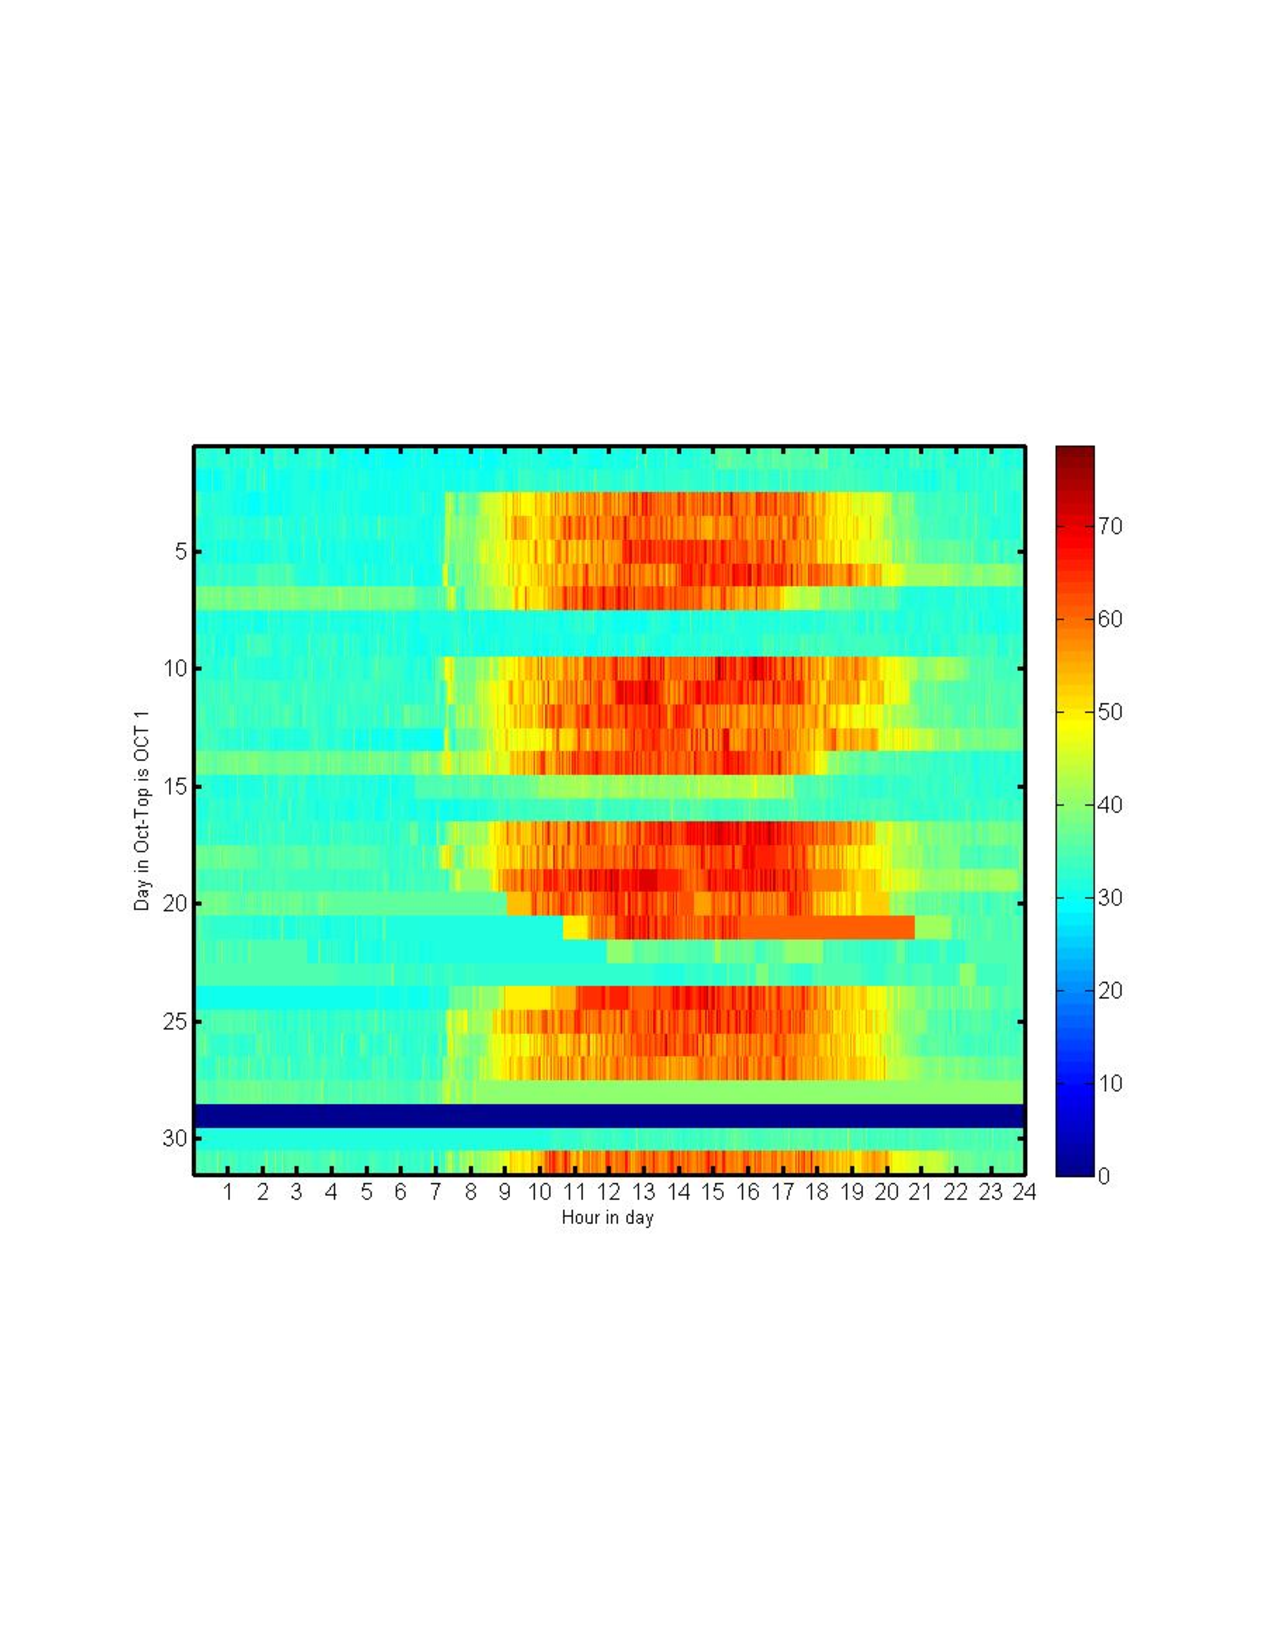
\includegraphics[scale=0.49]{figs/Aggregate_SDH_OCT_PLUG_LOADS}
\caption{Power heatmap generated from the data obtained from meters attached to plug-load devices throughout the building.  
Red zones are locations where the highest amount of power is being consumed.}
\label{fig:plugloadheatmap}
\end{center}
\end{figure}

Figure~\ref{fig:plugloadheatmap} was generated using actual live, plugload data throughout the day during the entire month
of October.  The x-axis shows the hour of the day, while the y-axis indicates the day in october.  This data was aggregated
over hourly period by summing all the plug-load data collected over that hour.  Notice the busiest times between 10am and 
about 6pm.  There's also a clear view of the weekends.

% \begin{figure*}[htb!]
% \begin{center}
% 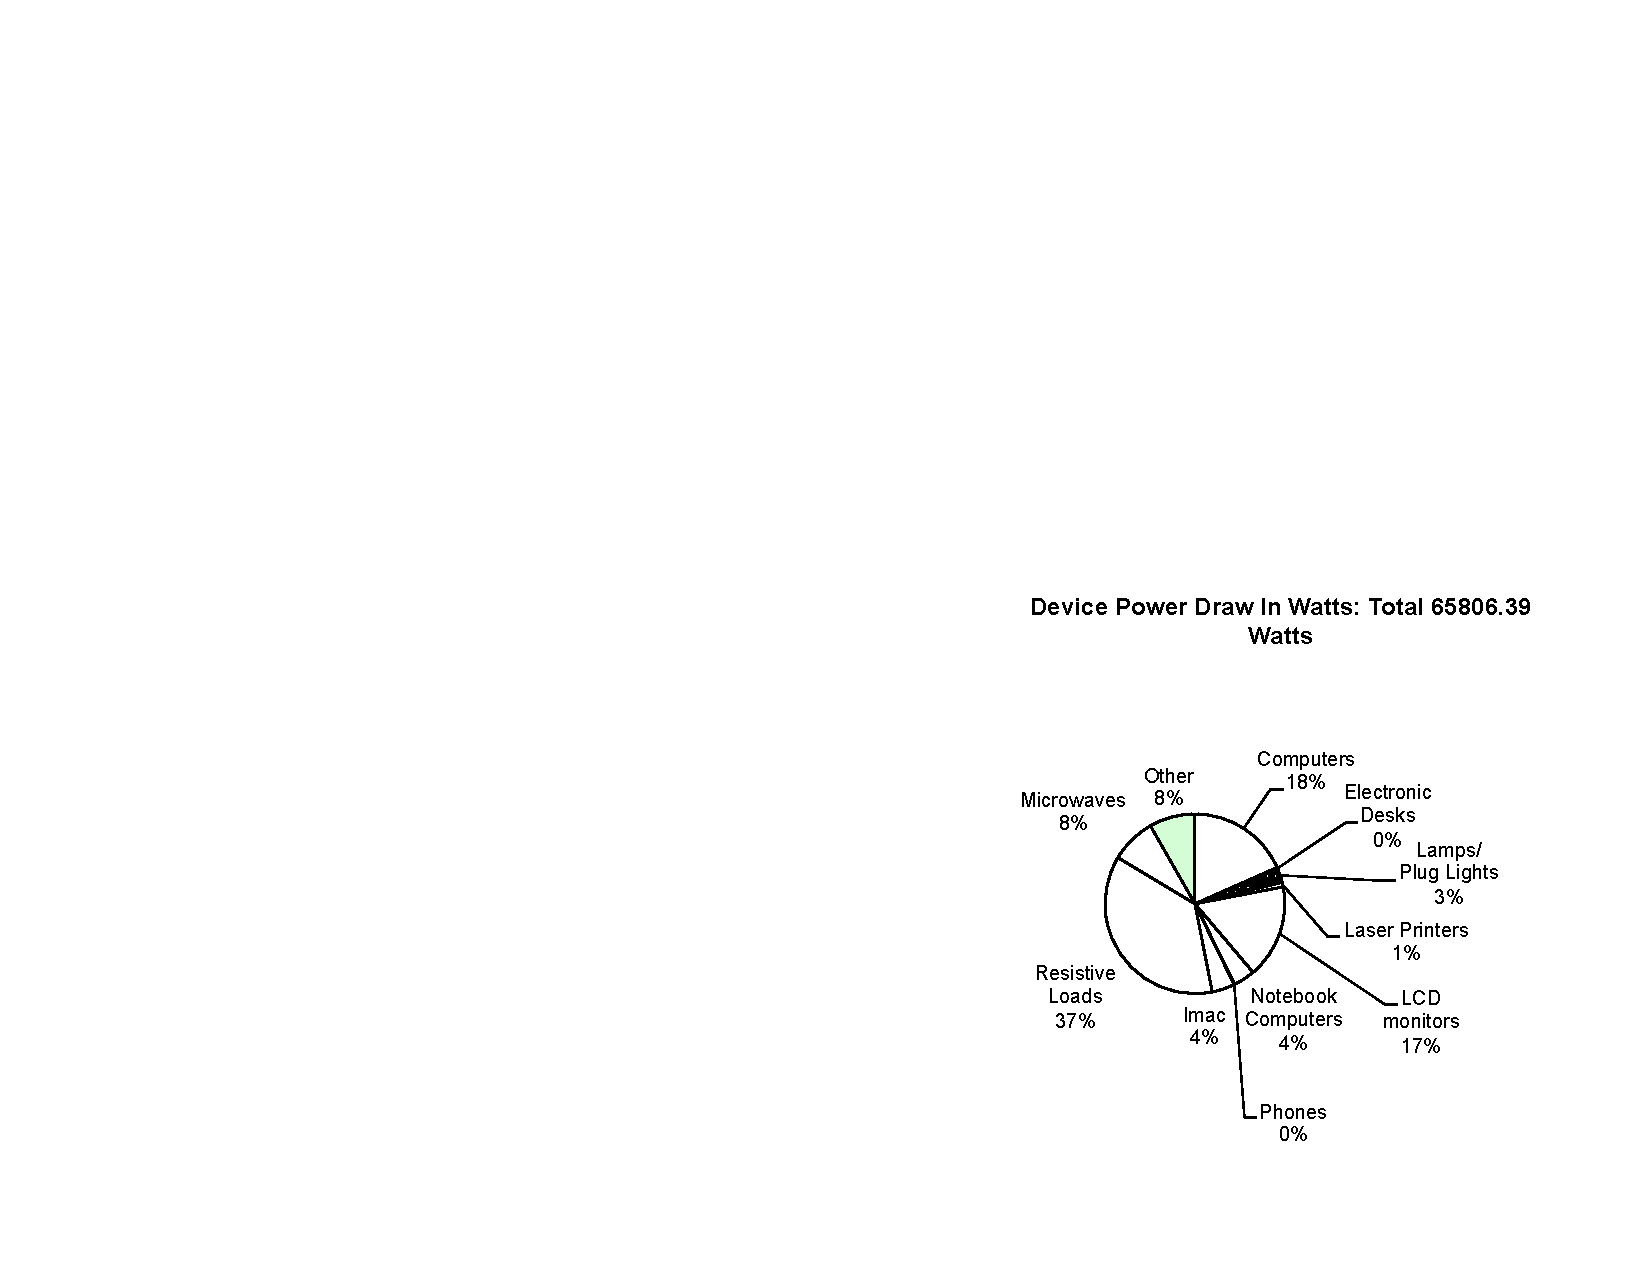
\includegraphics[scale=0.8]{figs/device_info02}
% \caption{}
% \label{channelcomp}
% \end{center}
% \end{figure*}

\begin{figure}[htb!]
\begin{center}
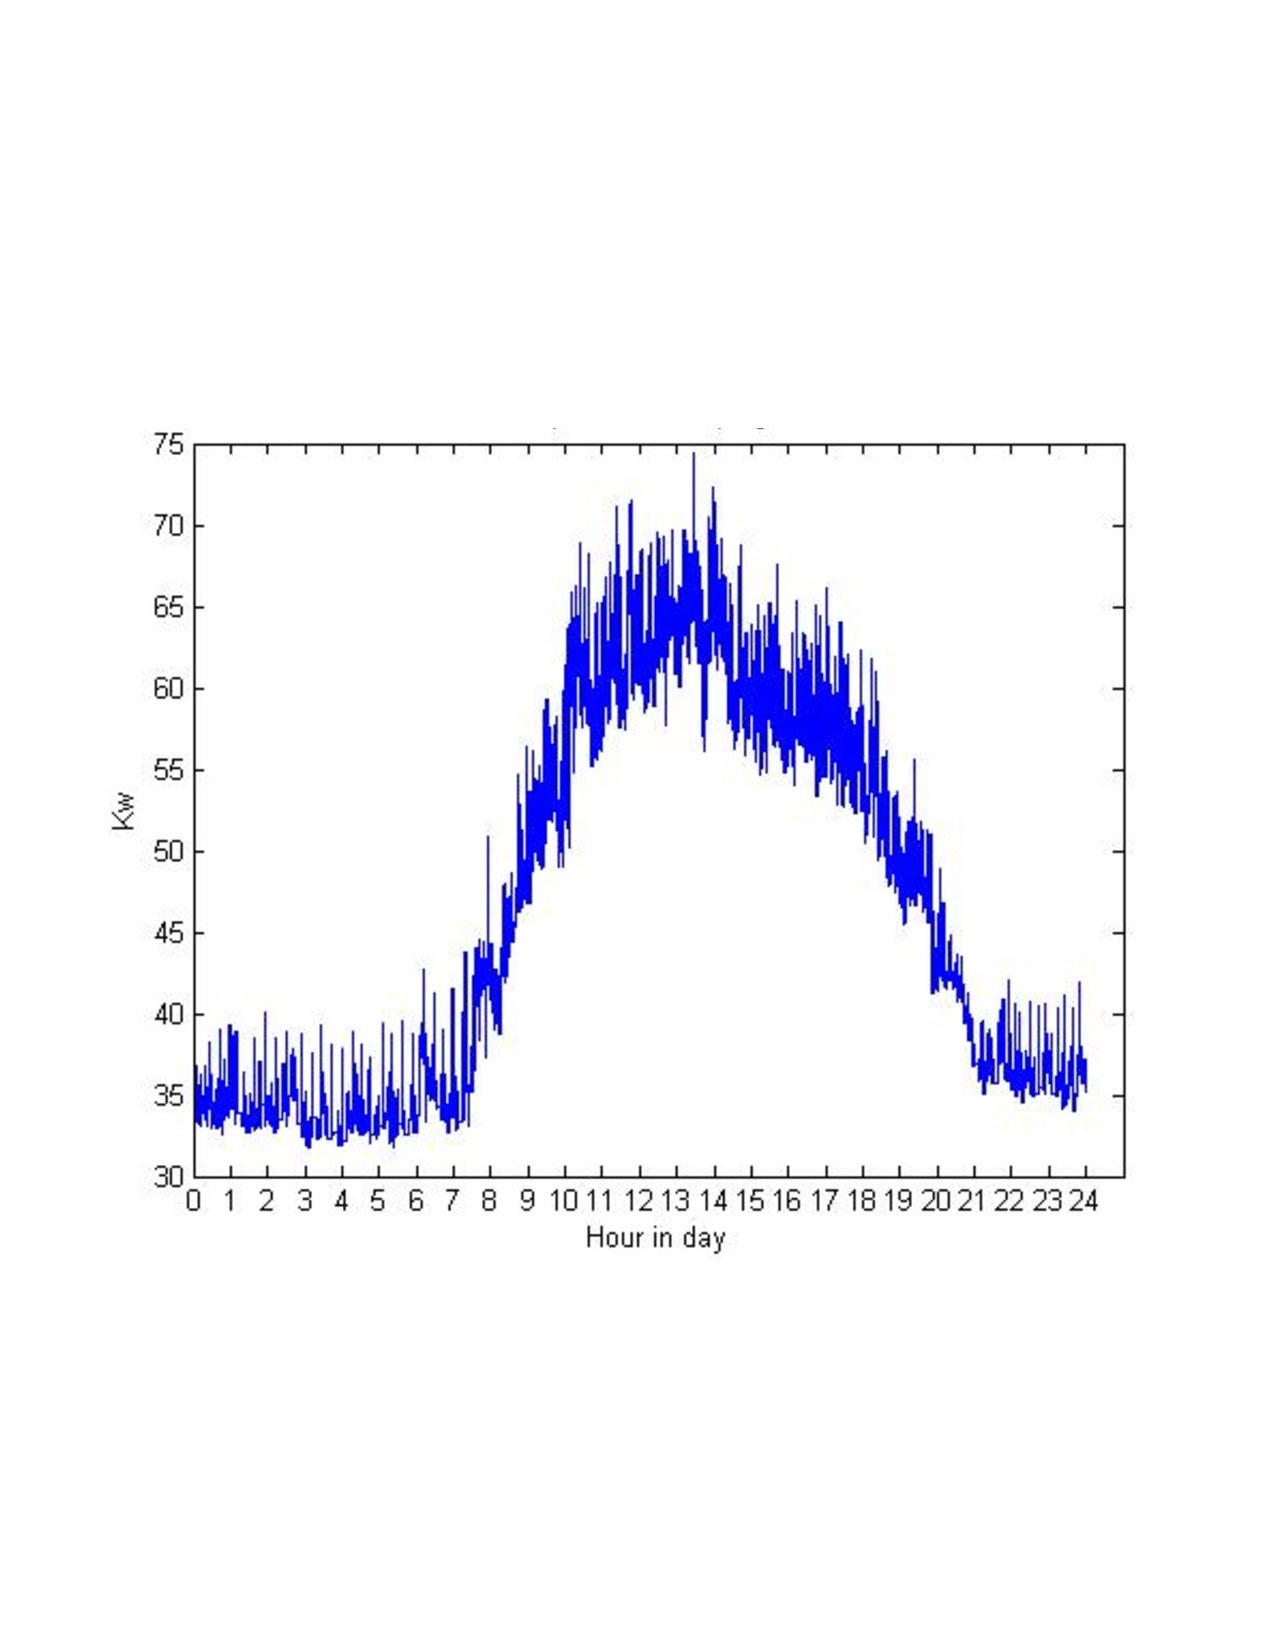
\includegraphics[scale=0.4]{figs/WholeOct12}
\caption{Whole building power draw on October 12th.}
\label{fig:wholebuilding}
\end{center}
\end{figure}

Figure~\ref{fig:wholebuilding} shows the whole building power-draw feed.  This meter was obtained through the building
management system and added to the audit.  Notice how the peak and low times correspond to the patterns observed
in the monthly plug-load heat map.

% \begin{figure}[htb!]
% \begin{center}
% 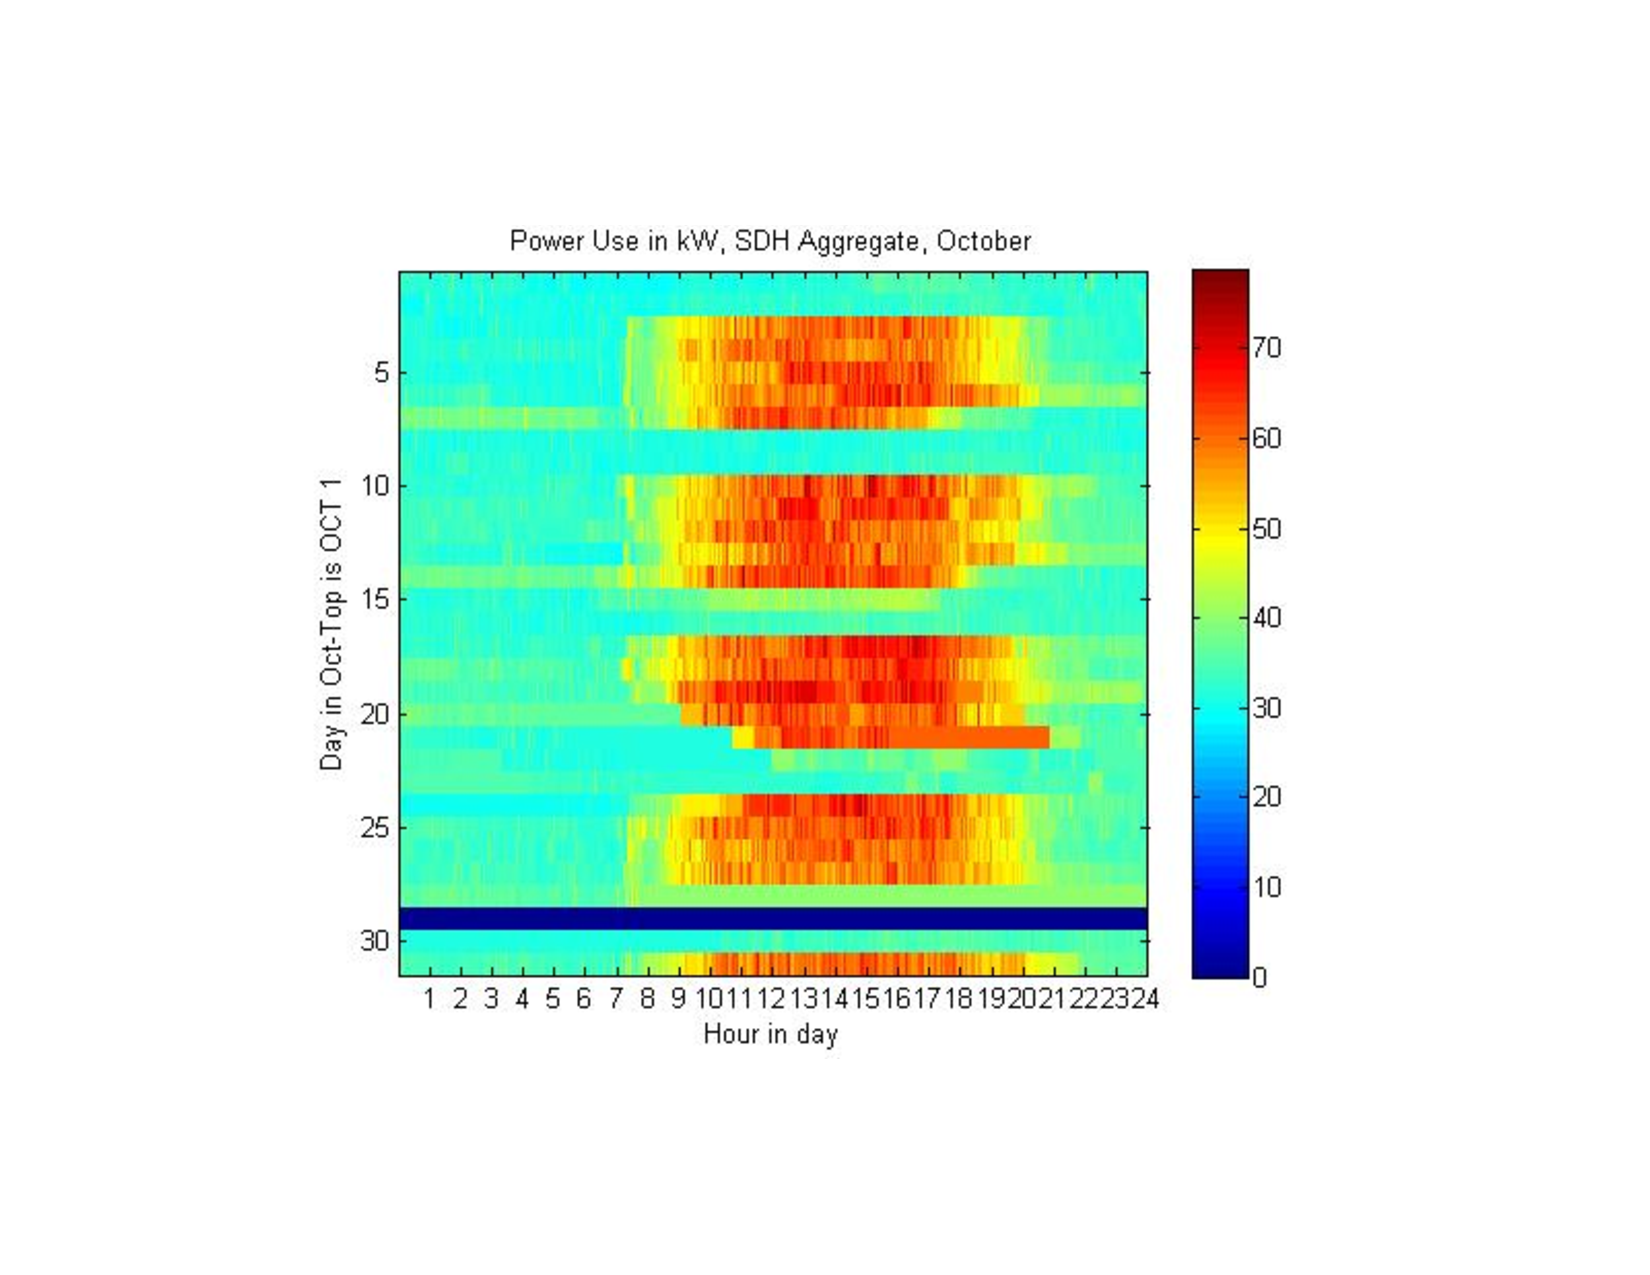
\includegraphics[scale=0.4]{figs/heatgrid}
% \caption{}
% \label{channelcomp}
% \end{center}
% \end{figure}

\begin{figure}[htb!]
\begin{center}
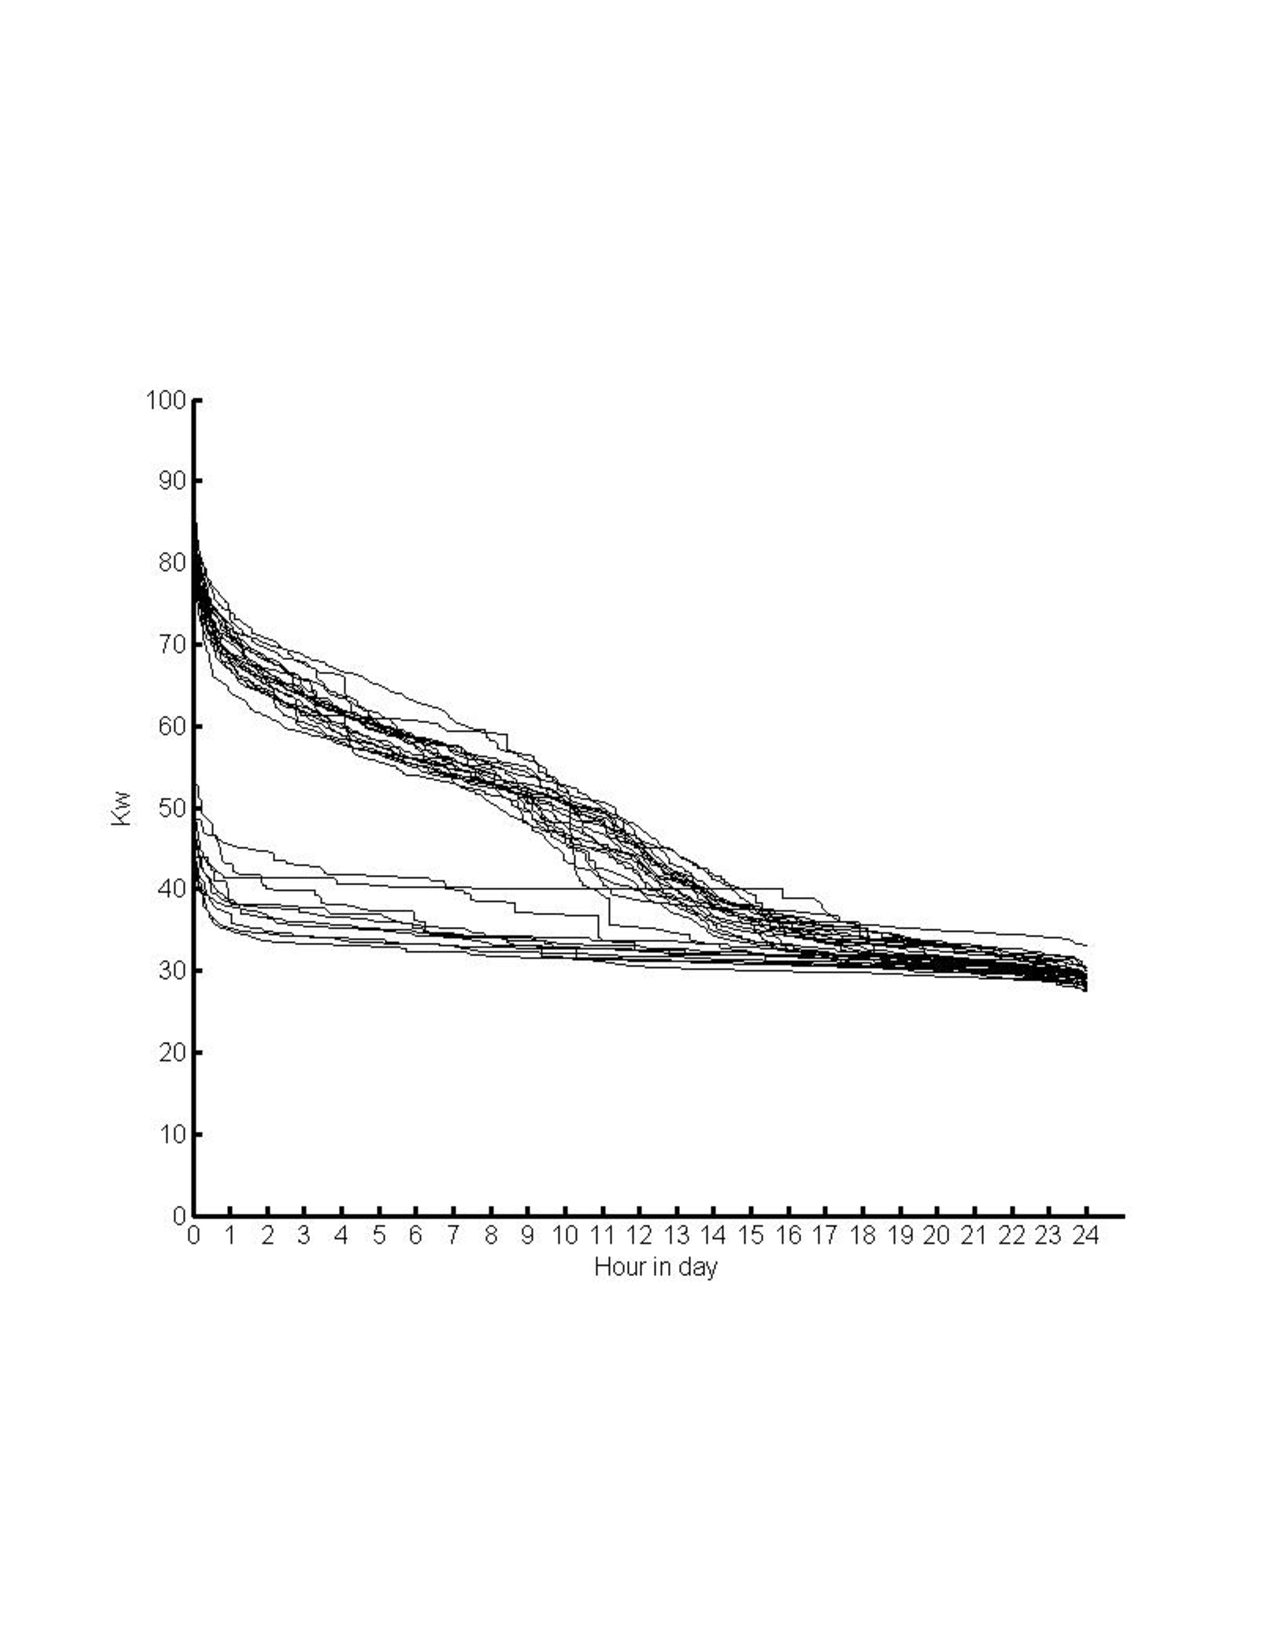
\includegraphics[scale=0.4]{figs/LoadDurationCurvesWholeBuildingBLACK}
\caption{Load duration curves.}
\label{fig:ldc}
\end{center}
\end{figure}

Figure~\ref{fig:ldc} shows the load duration curve for each day in the month of October.  The load duration
curve shows the number of hours in a 24-hour day that the load was at or above the level indicated on the 
y-axis.

\subsubsection{Issues}
Although many of the calculations are static and in large aggregates there were some fundamental challenges that
we encountered.  The first challenge is maintaining \emph{consistency} between the physical world and the virtual
representation of it.  About 16\% of the plug-load items we registered can be moved between locations by they owner
with relative frequency.  7\% (laptops) move quite often.  Maintaing of accurate view of what items are where
is a non-trivial with the right mechanisms in place.  Our approach in this case is to depend on the ubiquity of
smartphones and participants.  If a person moves an item from one location to another, they can swipe the item out
of the current location and swipe the item back in at the new location.  In addition, we take advantage of
natural usage patterns.  People tend to forget to swipe items out of their current location, so we leverage the
second swipe (swipe-in) to imply the first operation (swipe-out).  If the item was connected to a meter, we unbind the item
from the old meter before swiping the item out.  

We are currently working on adjusting the timestamp based on this action as well.
From the trace of the meter we can see when the item was unplugged (or turned off).  The sudden drop in power
reading could be used to mark the point of disconnection.  However, this only gets us part of the solution.  If the person
forgets multiple actions, it become more difficult to determine what has occurred.  For example, if a lamp is plugged
into a meter in room 1 and they unplug it from the meter, plug another device into it, and move the lamp to
another location, the unplug time is not clear.  If the new device draws power, we cannot tell the difference between
the trace generated from the new device versus the old device.  This is a non-intrusive load-trace classification
problem and beyond the scope of the current project.

% \begin{itemize}
% %\item Context tracking:  Localization through a swipe or implicit location change through natural action
% \item tracking mobile users
% \item tracking mobile objects
% 	\begin{itemize}
% 	\item devices
% 	\item meters
% 	\end{itemize}
% \end{itemize}